\begin{enumerate}[label=\thechapter.\arabic*,ref=\thechapter.\theenumi]

\item Consider a unity-gain negative feedback system consisting of the plant $G\brak{s}$  and a proportional-integral controller. Let the proportional gain and integral
gain be 3 and 1, respectively. For a unit step reference input, the final values of the
controller output and the plant output, respectively, are
\begin{align}
    G\brak{s} = \frac{1}{\brak{s-1}} \notag
\end{align}\hfill (GATE EE 2023)\\
\solution 
% \iffalse
\let\negmedspace\undefined
\let\negthickspace\undefined
\documentclass[journal,12pt,twocolumn]{IEEEtran}
\usepackage{cite}
\usepackage{amsmath,amssymb,amsfonts,amsthm}
\usepackage{algorithmic}
\usepackage{graphicx}
\usepackage{textcomp}
\usepackage{xcolor}
\usepackage{txfonts}
\usepackage{listings}
\usepackage{enumitem}
\usepackage{mathtools}
\usepackage{gensymb}
\usepackage{comment}
\usepackage[breaklinks=true]{hyperref}
\usepackage{tkz-euclide} 
\usepackage{listings}
\usepackage{gvv}                                        
\def\inputGnumericTable{}                                 
\usepackage[latin1]{inputenc}                                
\usepackage{color}                                            
\usepackage{array}                                            
\usepackage{longtable}                                       
\usepackage{calc}                                             
\usepackage{multirow}                                         
\usepackage{hhline}                                           
\usepackage{ifthen}                                           
\usepackage{lscape}
\newtheorem{theorem}{Theorem}[section]
\newtheorem{problem}{Problem}
\newtheorem{proposition}{Proposition}[section]
\newtheorem{lemma}{Lemma}[section]
\newtheorem{corollary}[theorem]{Corollary}
\newtheorem{example}{Example}[section]
\newtheorem{definition}[problem]{Definition}
\newcommand{\BEQA}{\begin{eqnarray}}
\newcommand{\EEQA}{\end{eqnarray}}
\newcommand{\define}{\stackrel{\triangle}{=}}
\theoremstyle{remark}
\newtheorem{rem}{Remark}
\begin{document}
\parindent 0px

\bibliographystyle{IEEEtran}
\vspace{3cm}

\title{Assignment\\[1ex]GATE-EC-39}
\author{EE23BTECH11034 - Prabhat Kukunuri$^{}$% <-this % stops a space
}
\maketitle
\newpage
\bigskip

\renewcommand{\thefigure}{\theenumi}
\renewcommand{\thetable}{\theenumi}
\section{Question}
Consider the circuit shown in the figure with input V(t) in volts.The sinusoidal steady state current I(t) flowing through the circuit is shown graphically(where t is in seconds). The circuit element Z can be\rule{1.5cm}{0.15mm}.
\begin{enumerate}
    \item a capacitor of 1 F
    \item an inductor of 1 H
    \item a capacitor of $\sqrt{3}$ H
    \item an inductor of $\sqrt{3}$ H
\end{enumerate}
\begin{figure}[ht]
    \centering
    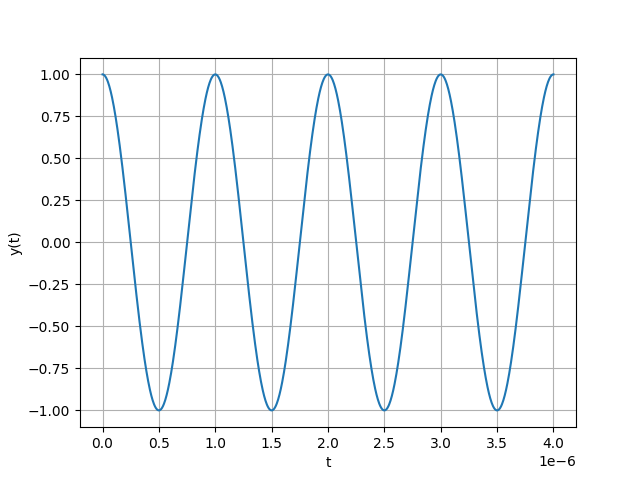
\includegraphics[width=\columnwidth]{figs/Figure_1.png}
    \label{fig:GATE.2022.EC.39.1}
\end{figure}
\solution\\
\begin{table}[h]
    \centering
    \begin{tabular}{|p{2cm}|p{2.80cm}|p{2.70cm}|}
    \hline
    Symbol&Value&Description\\ \hline
    $$x(n)$$&$$(x(0)+nd)u(n)$$&$$n^{th}$$ term of an A.P\\ \hline
    $$x(0)$$&$$x(0)$$&$1^{st}$ term of the A.P\\ \hline
    $$d$$&$$d$$&Common difference\\ \hline
    $$y(n)$$&$$x(n)\ast u(n)$$&Sum of n terms of an AP\\ \hline
    $$a$$&$$y(p-1)$$&Sum of first p terms of the AP\\ \hline
    $$b$$&$$y(q-1)$$&Sum of first q terms of the AP\\ \hline
    $$c$$&$$y(r-1)$$&Sum of first r terms of the AP\\ \hline
\end{tabular}
    \caption{Variable description}
    \label{tab:GATE.2022.EC.39.1}
\end{table}\\
The current through the circuit can be expressed as
\begin{align}
    I(t)=\sin\brak{t-\frac{\pi}{4}}
\end{align}
Since, the voltage seems to be leading the current the circuit element z is an inductor with inductance L.\\
Applying KVL in the circuit,
\begin{align}
    R.I\brak{t}+L\frac{dI\brak{t}}{dt}=sin\brak{t}
\end{align}
Applying Fourier transform to the differential equation,
\begin{align}
    &R.I\brak{s}+sL.I\brak{s}-\frac{1}{s^2+1}=0\\
    &I\brak{s}\brak{R+sL}=\frac{1}{s^2+1}\\
    &\sin\brak{at+b}\system{L}\frac{a\cos\brak{b}+s\sin\brak{b}}{a^{2}+s^{2}}\\
    &\sin\brak{t-\frac{\pi}{4}}\system{L}\frac{1-s}{2\brak{s^2+1}}\\
    &\frac{1-s}{2\brak{s^2+1}}\brak{R+sL}=\frac{1}{s^2+1}
\end{align}
Upon plugging in R=1$\ohm$,
\begin{align}
   L=\frac{1}{s}
\end{align}
Applying inverse Laplace,
\begin{align}
    L=1H
\end{align}

Appendix\\
Laplace transform of $\sin\brak{at+b}$ is as follows,
\begin{align}
    &\sin\brak{at+b}\system{L}\int_{0}^{\infty}\sin\brak{at+b}e^{-st}dt\\
    &\int_{0}^{\infty}\sin\brak{at+b}e^{-st}dt=\cos{b}\int_{0}^{\infty}\sin\brak{at}e^{-st}dt+\sin{b}\int_{0}^{\infty}\cos\brak{at}e^{-st}dt\\
    &\int_{0}^{\infty}\cos\brak{at}e^{-st}dt=\frac{e^{-st}}{a}sin{at}\Bigg|_{0}^{\infty}+\frac{s}{a}\int_{0}^{\infty}\sin\brak{at}e^{-st}dt\\
    &\int_{0}^{\infty}\cos\brak{at}e^{-st}dt=\frac{s}{a}\int_{0}^{\infty}\sin\brak{at}e^{-st}dt\label{eq:GATE.2022.EC.39.2}\\
    &\int_{0}^{\infty}\cos\brak{at}e^{-st}dt=\frac{s}{a}\brak{\frac{-e^{-st}}{a}cos{at}\Bigg|_{0}^{\infty}+\frac{s}{a}\int_{0}^{\infty}\cos\brak{at}e^{-st}dt}\\
    &\int_{0}^{\infty}\cos\brak{at}e^{-st}dt=\frac{s}{a^2}+\frac{s^2}{a^2}\int_{0}^{\infty}\cos\brak{at}e^{-st}dt
\end{align}
\begin{align}
    &\int_{0}^{\infty}\cos\brak{at}e^{-st}dt=\frac{s}{s^2+a^2},s>0
\end{align}
From \eqref{eq:GATE.2022.EC.39.2} we can say,
\begin{align}
    &\int_{0}^{\infty}\sin\brak{at}e^{-st}dt=\frac{a}{s^2+a^2},s>0\\
    &\therefore \sin\brak{at+b}\system{L}\frac{s\sin{b}+a\cos{b}}{s^2+a^2}
\end{align}
\end{document}

\newpage

\item Level \brak{h} in a steam boiler is controlled by manipulating the flow rate \brak{F} of the break-up(fresh) water using a proportional \brak{P} controller. The transfer function between the output and the manipulated input is   \\
$$ \frac{h\brak{s}}{F\brak{s}}=\frac{0.25\brak{1-s}}{s\brak{2s+1}} $$   \\
The measurement and the valve transfer functions are both equal to 1. A process engineer wants to tune the controller so that the closed loop response gives the decaying oscillations under the servo mode. Which one of the following is the CORRECT value of the controller gain to be used by the engineer? \\
\begin{enumerate}[label=(\alph*)]
    \item $0.25$
    \item $2$
    \item $4$
    \item $6$
\end{enumerate}

\solution
\newpage
\item \iffalse
\let\negmedspace\undefined
\let\negthickspace\undefined
\documentclass[journal,12pt,twocolumn]{IEEEtran}
\usepackage{cite}
\usepackage{amsmath,amssymb,amsfonts,amsthm}
\usepackage{algorithmic}
\usepackage{graphicx}
\usepackage{textcomp}
\usepackage{xcolor}
\usepackage{txfonts}
\usepackage{listings}
\usepackage{enumitem}
\usepackage{mathtools}
\usepackage{gensymb}
\usepackage{comment}
\usepackage[breaklinks=true]{hyperref}
\usepackage{tkz-euclide} 
\usepackage{listings}
\usepackage{gvv}                                        
\def\inputGnumericTable{}                                 
\usepackage[latin1]{inputenc}                                
\usepackage{color}                                            
\usepackage{array}                                            
\usepackage{longtable}                                       
\usepackage{calc}                                             
\usepackage{multirow}                                         
\usepackage{hhline}                                           
\usepackage{ifthen}                                           
\usepackage{lscape}
\usepackage{placeins}
\usepackage{xparse}


\newtheorem{theorem}{Theorem}[section]
\newtheorem{problem}{Problem}
\newtheorem{proposition}{Proposition}[section]
\newtheorem{lemma}{Lemma}[section]
\newtheorem{corollary}[theorem]{Corollary}
\newtheorem{example}{Example}[section]
\newtheorem{definition}[problem]{Definition}
\newcommand{\BEQA}{\begin{eqnarray}}
\newcommand{\EEQA}{\end{eqnarray}}
\newcommand{\define}{\stackrel{\triangle}{=}}
\theoremstyle{remark}
\newtheorem{rem}{Remark}

\graphicspath{ {./figs/} } 

\begin{document}

\bibliographystyle{IEEEtran}
\vspace{3cm}

\Large\title{GATE ME 30}
\large\author{EE23BTECH11032 - Kaustubh Parag Khachane $^{*}$% <-this % stops a space
}
\maketitle
\newpage
\bigskip

\renewcommand{\thefigure}{\theenumi}
\renewcommand{\thetable}{\theenumi}

\large\textbf{Question GATE ME 30} :\\
\fi
The figure shows a block of mass m = 20 kg attached to a pair of identical linear springs, each having a spring constant k = 1000 N/m. The block oscillates on a frictionless horizontal surface. Assuming free vibrations, the time taken by the block to complete ten oscillations is \rule{1cm}{0.15mm} seconds . (Rounded off to two decimal places) Take $\pi$ = 3.14.\hfill{GATE ME 30}

\begin{figure}[!ht]
\centering
\begin{center}
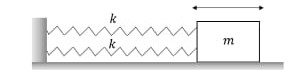
\includegraphics[width=\columnwidth]{2023/ME/30/figs/questiondiagram}
\end{center}
%\caption{Diagram for GATE ME Question 30}
\end{figure}


\item A system has transfer function
 \[\frac{Y(s)}{X(s)}=\frac {s-\pi}{s+\pi}\]
 let $u(t)$ be the unit step function.The input $x(t)$ that results in a steady-state output $y(t)=sin(\pi t)$ is \underline{\quad}.\hfill (GATE IN 2023)\\
 \solution
 \newpage
 
\end{enumerate}
